\documentclass[10pt, conference, compsocconf]{IEEEtran}

\usepackage{capt-of}
\usepackage{graphicx}
\usepackage{subfig}
\usepackage{booktabs}
\usepackage{multirow}
\usepackage{siunitx}
\usepackage{multicol}
\usepackage{array}
\usepackage{amsmath}
\newcommand{\BIBdecl}{\setlength{\itemsep}{0.0 em}}


\newcommand{\nltable}[2][c]{%
  \begin{tabular}[#1]{@{}c@{}}#2\end{tabular}}
\newcommand{\wave}{\raise.17ex\hbox{$\scriptstyle\mathtt{\sim}$}}

\newcolumntype{C}[1]{>{\centering\let\newline\\\arraybackslash}m{#1}}

\begin{document}
\bstctlcite{IEEEexample:BSTcontrol}

\title{MPEC : Distributed Matrix Multiplication Performance Estimator \\for Machine Learning Jobs in Cloud Computing}
%  Remark: Please note that most journals do not allow the use of abbreviations in titles. Please check the target journal guidelines to verify the same and revise accordingly.

\author{\IEEEauthorblockN{Myungjun Son}
\IEEEauthorblockA{Department of Computer Science\\
Kookmin University\\
Seoul, South Korea\\
smj8612@kookmin.ac.kr}
\and
\IEEEauthorblockN{Kyungyong Lee}
\IEEEauthorblockA{Department of Computer Science\\
Kookmin University\\
Seoul, South Korea\\
leeky@kookmin.ac.kr}
}

% make the title area
\maketitle

\begin{abstract}
  Matrix multiplication is an important kernel task in many machine learning algorithms. As the size of input datasets increase, multiple workloads are analyzed in large-scale distributed cloud computing environments. Furthermore, understanding the characteristics of a distributed matrix multiplication task is essential for running machine learning jobs in the cloud. Herein, we propose matrix multiplication performance estimator for cloud computing \textbf{MPEC}, a method to predict the latency of matrix multiplication of various sizes and shapes in a distributed cloud computing environment. We first characterize the overhead of a distributed matrix multiplication task and propose features to model the latency of a task with different input types. Using the proposed features, a latency prediction model is developed by applying a data mining algorithm and a parameter optimization step iteratively. In experiments with 236 distinct types of matrix multiplications on diverse cloud instances running Apache Spark, we confirm that the proposed method can model the latency of various types of matrix multiplication tasks effectively and capture the non-linear interactions among the proposed features. A comparison with the state-of-the-art cloud computing performance predictor reveals that MPEC provides 16\% greater accuracy for a distributed matrix multiplication task and confirms the uniqueness of the distributed matrix multiplication workload.
\end{abstract}

\IEEEpeerreviewmaketitle

\section{Introduction}\label{sec:intro}
Many big data analysis systems are deployed in cloud computing environments to process increasingly large datasets while guaranteeing stable operations, scalability, and fault-tolerance from the viewpoint of infrastructure. To satisfy application demands from distinct use cases, cloud computing service providers offer various types of configuration instances and many big data systems are deployed in a scale-out manner. In such environments, managing distributed compute resources, datasets, and programming is challenging. To relieve the burden of managing distributed resources and allow application developers to focus on critical tasks, many systems that provide simple and easy interfaces to handle large-scale datasets have been proposed, e.g., Apache Spark~\cite{spark}.

Data mining algorithms are used to extract valuable information from massive datasets, and in many machine learning algorithms, matrix multiplication is the core computation kernel. For example, in recommendation systems, the core computation kernel of matrix factorization algorithms, such as SVD and NMF~\cite{nmf}, is matrix-matrix multiplication. Matrix-vector multiplication is the core kernel of the PageRank algorithm when using the power method to obtain principle eigenvectors~\cite{pagerank}. To build a cost-efficient cloud environment wherein machine learning tasks can be performed with a distributed matrix computation kernel, it is crucial to estimate the overhead of kernel tasks with distinct matrix sizes and shapes.

To understand the characteristics of matrix multiplication performance in a distributed cloud computing environment, we analyzed the performance of dense matrix multiplication with diverse input sizes and formations on distinct cloud computing instances. In the experiments, we multiplied two square matrices (10000, 20000, and 30000 rows) on AWS EC2 \textit{R4, C4, G2} instances with a size of \textit{2xlarge}. We used the Apache Spark MLlib BlockMatrix library~\cite{spark-mm} to conduct the experiments with four machines with OpenBLAS installed.

\begin{figure}[t]
  \centering
  \subfloat[Different instance types]{\label{fig:different-instance-types}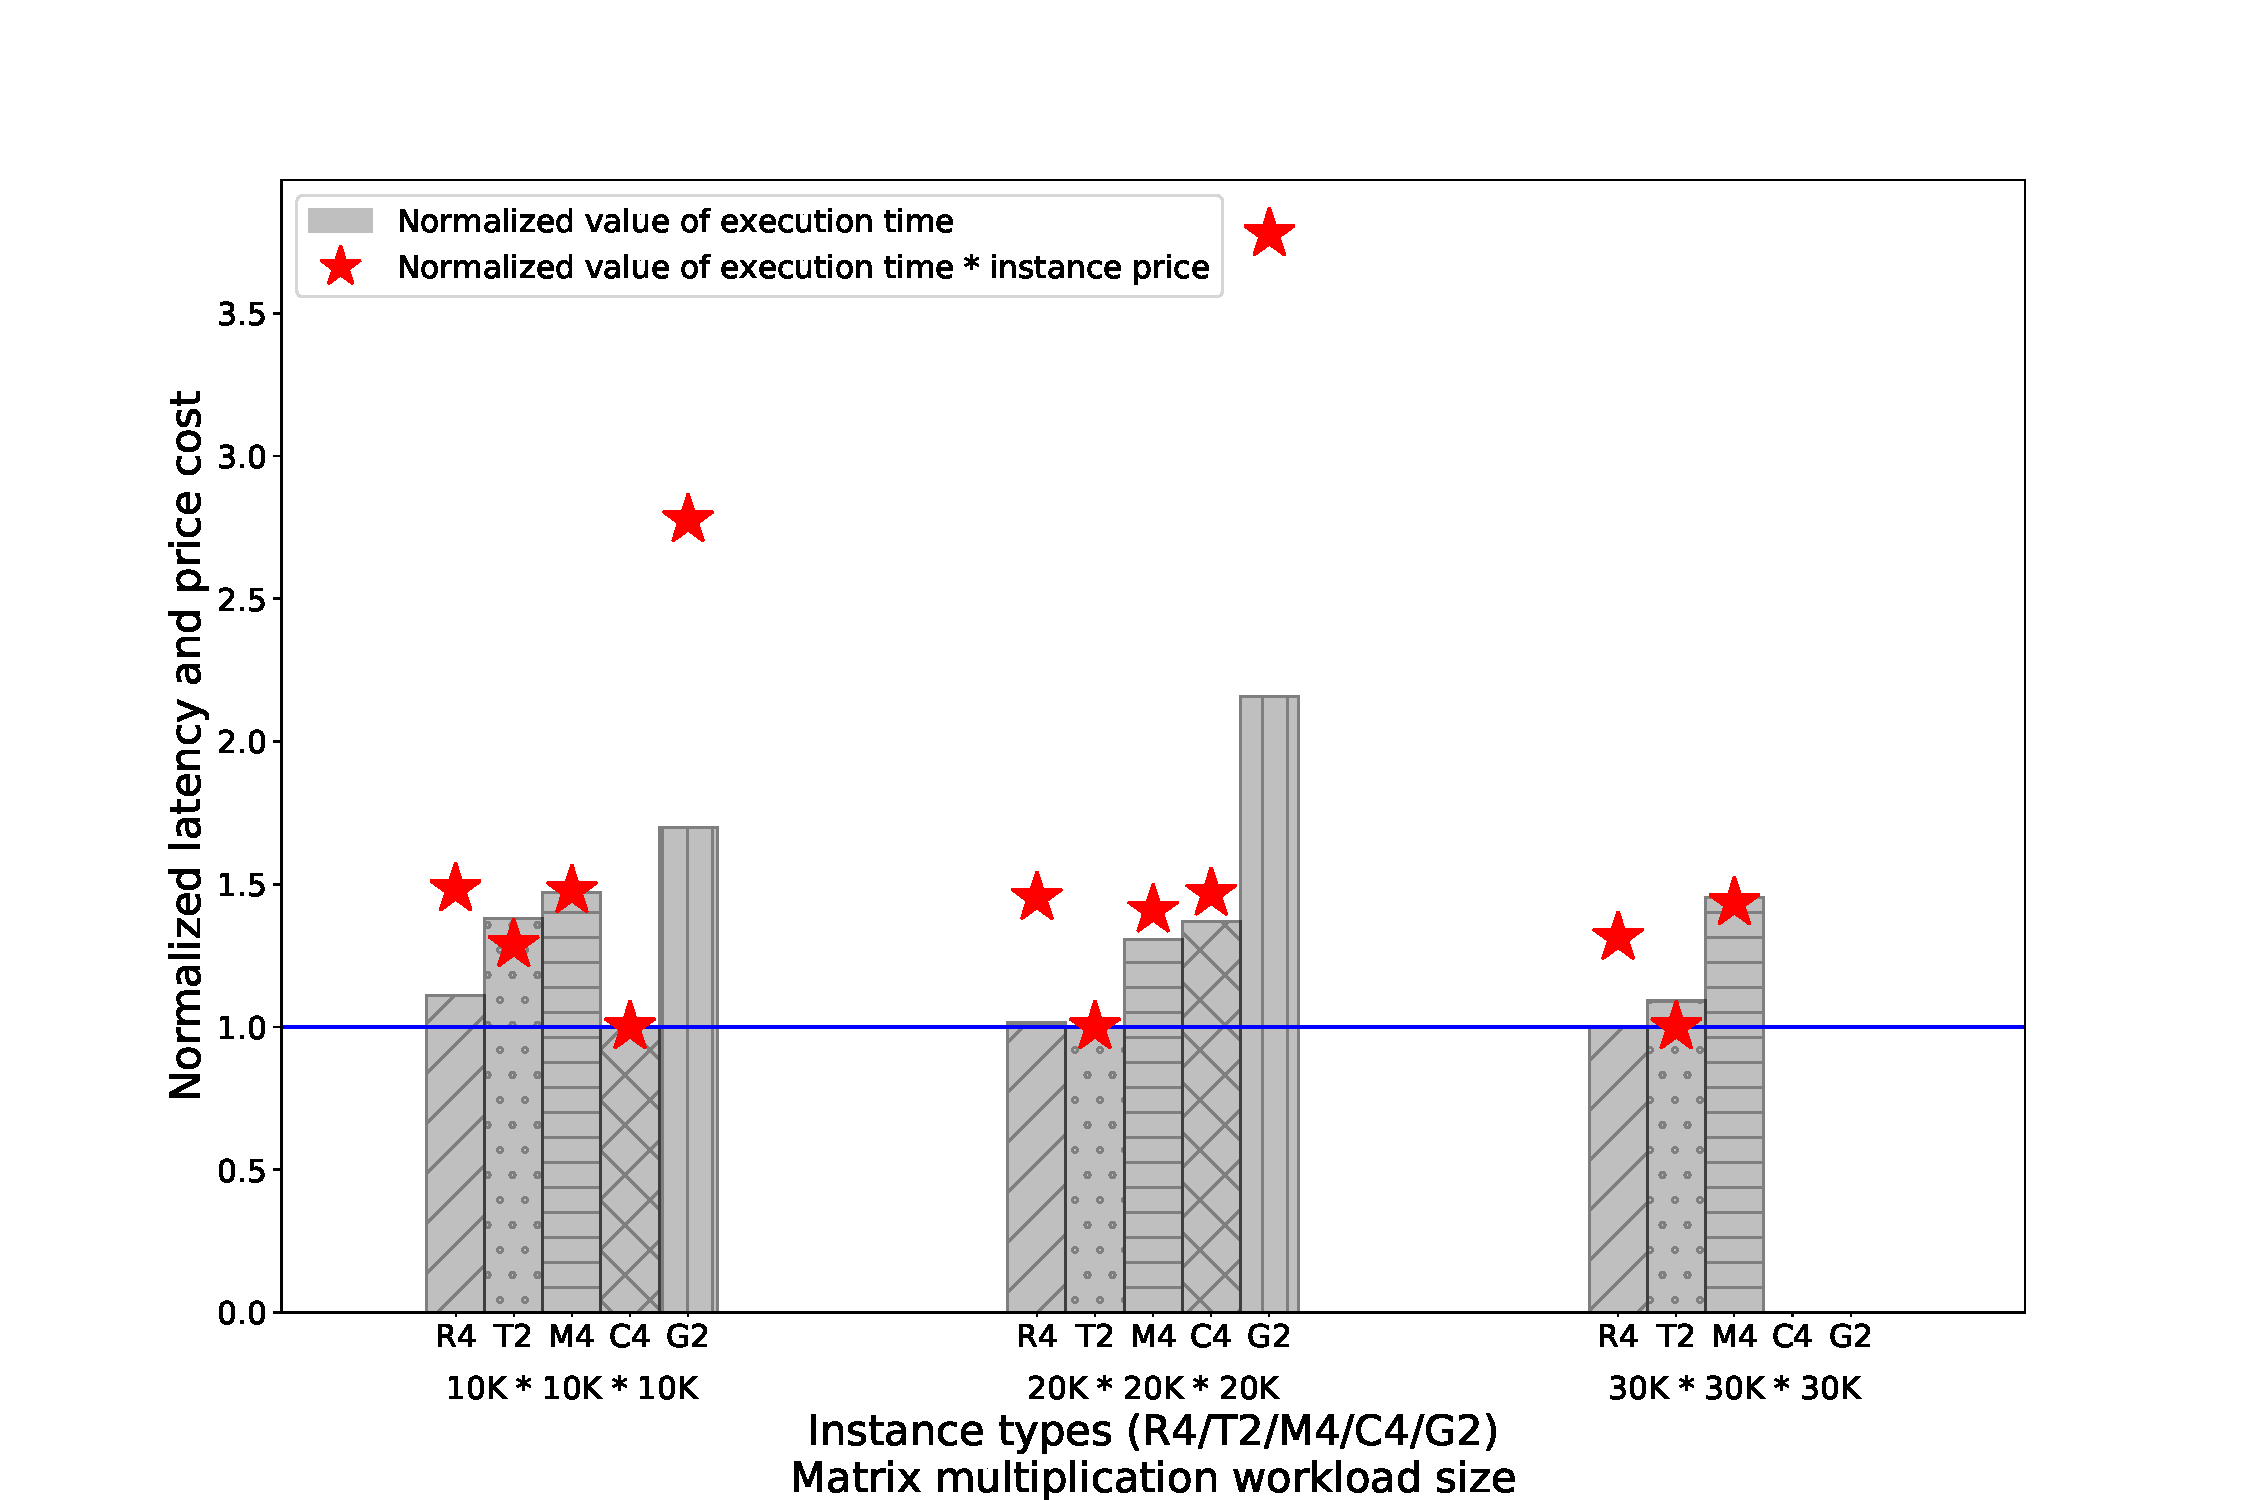
\includegraphics[width=4.5cm,height=4.5cm]{figures/instance-2xl-compare.pdf}}\hfil\hfil\hfil\hfil\hfil\hfil\hfil\hfil\hfil\hfil\subfloat[Different matrix shapes]{\label{fig:different-matrix-shapes}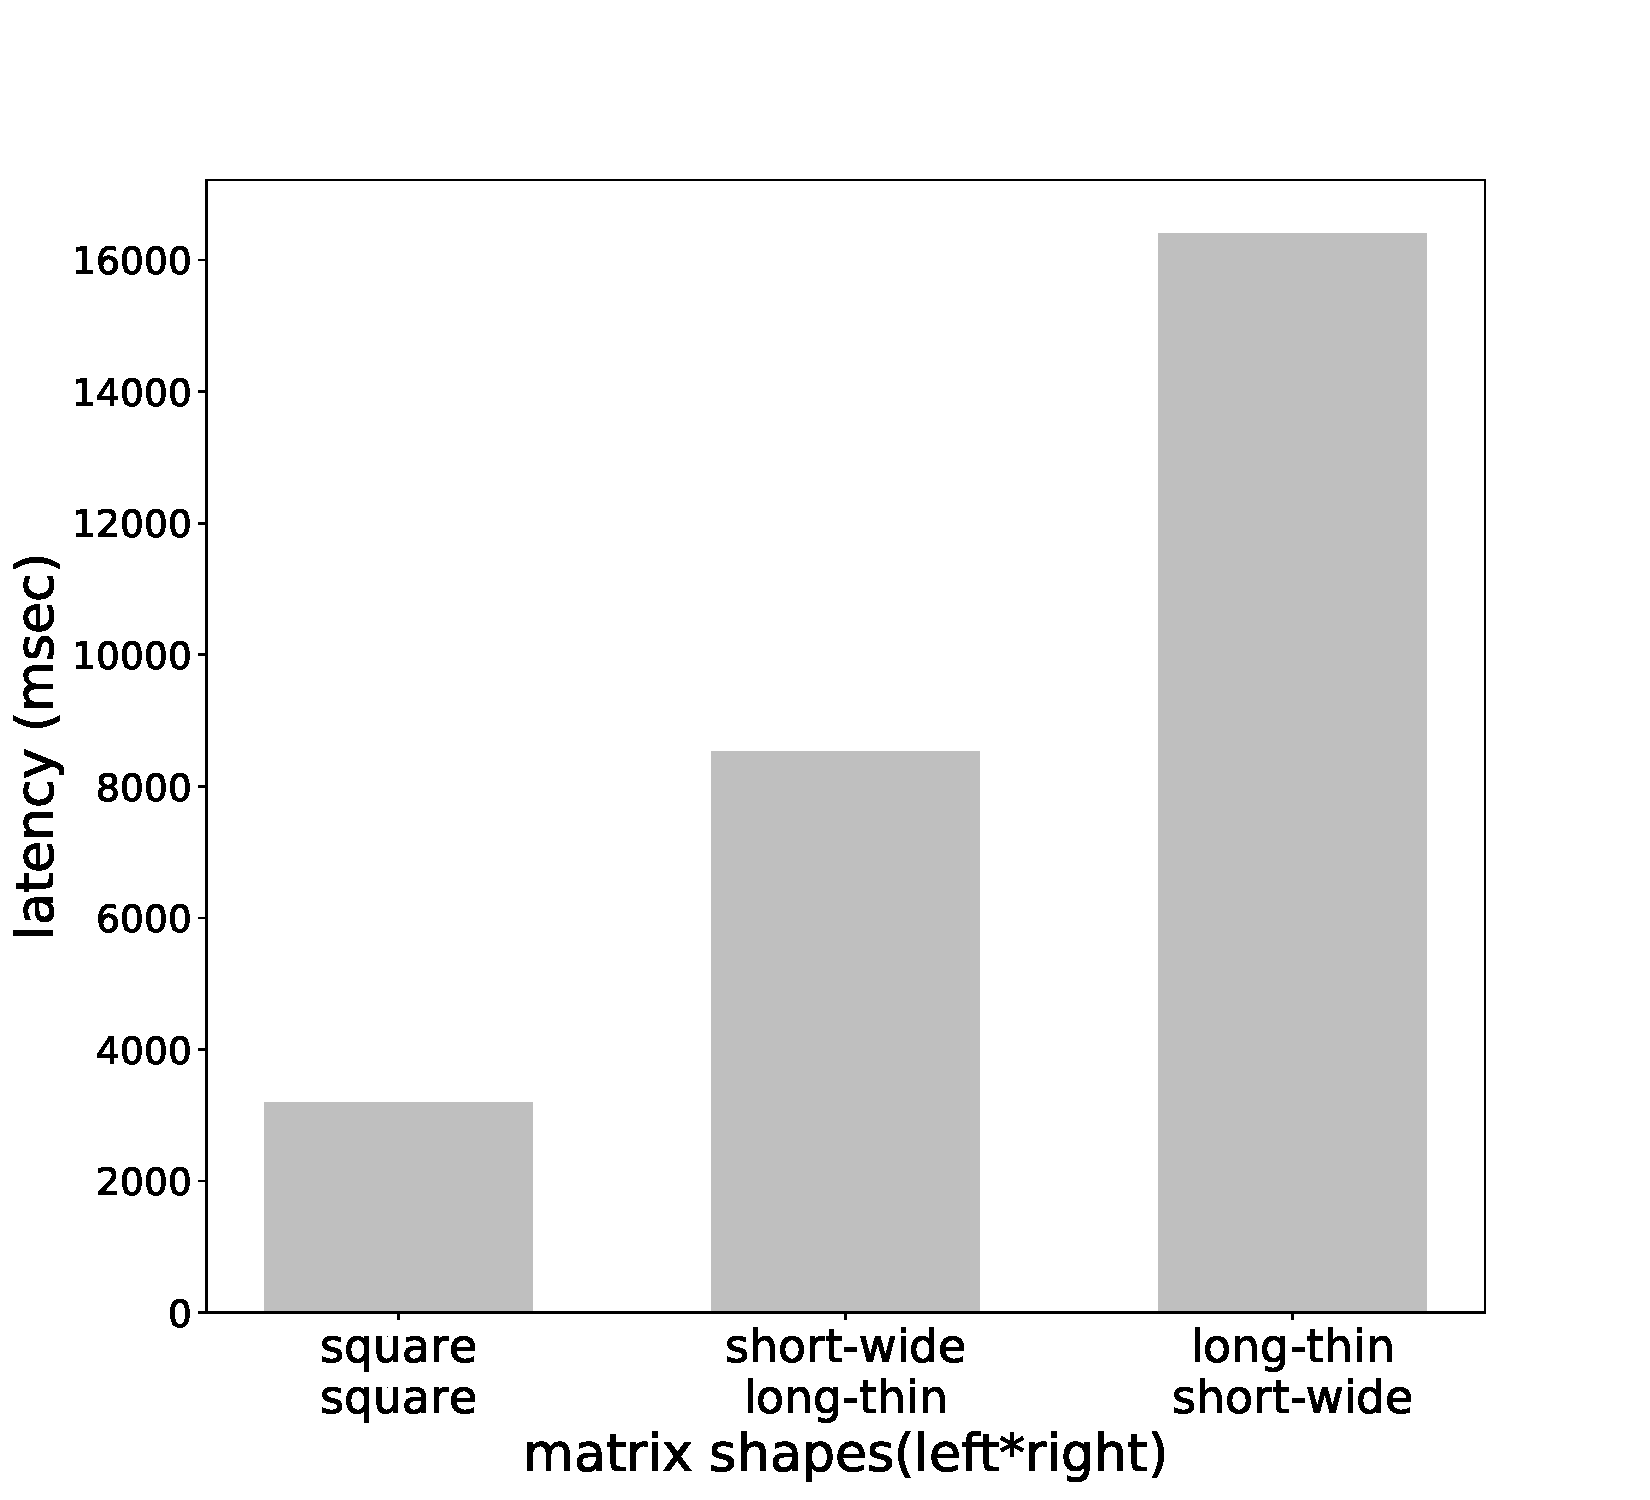
\includegraphics[width=4cm, height=4.5cm]{figures/matrix-multiplication-different-shape.pdf}}
  \caption{\label{fig:instance-blocks-sizes-compare}Normalized value of latency with different instance types and input matrix shapes (lower values are better)}
\end{figure}

In Figure~\ref{fig:different-instance-types}, the gray bar indicates shows the normalized latency of the fastest completing instance type. As shown in the figure, when the input matrix size differs, the best performing instance type differs. If we consider the price of each instance, the performance difference increases further (red star). Furthermore, as shown in Figure~\ref{fig:instance-blocks-sizes-compare}, the multiplication of two non-square matrices exhibits significantly different performance in comparison with that of square matrix multiplication even when the number of multiplication operations is the same, i.e., the number of left matrix rows $\times$ left matrix columns $\times$ right matrix columns. From the results shown in Figure~\ref{fig:instance-blocks-sizes-compare}, it is evident that estimating the latency of distributed matrix multiplication tasks with different matrix sizes and shapes is challenging.

Despite the importance of matrix multiplication in machine learning, comprehensive performance analyses and modeling in a distributed cloud computing environment have not been undertaken. Some methods, e.g., Ernest~\cite{ernest}, CherryPick~\cite{cherrypick}, and PARIS~\cite{paris}  focus on predicting machine learning task performance in a cloud computing environment. These methods rely on scale-based sampling to estimate the latency to complete a task with the entire original input dataset and show sufficient accuracy for some machine learning tasks. However, they show poor accuracy for predicting the latency of distributed matrix multiplication tasks because they fail to capture the complexity of distributed matrix computation. Many studies have investigated performance optimization, modeling, and prediction on a single machine with multiple cores using hardware-optimized libraries, e.g., OpenBLAS. However, these studies did not consider network and I/O overhead, which can be significant in a distributed cloud computing environment.

In this paper, we propose matrix multiplication performance estimator for cloud computing (MPEC), a method to predict the latency of matrix multiplication of arbitrary shapes and sizes using various cloud computing resource configurations. To represent the characteristics of distributed matrix multiplication tasks, such as the total number of multiplication operations, shuffle overhead, and output matrix size, the proposed MPEC employs eight features for modeling the task latency of distributed matrix multiplication. To determine the optimal hyperparameters for minimizing the prediction error, the proposed features are used to construct a model using a gradient boosting (GB) regressor, followed by Bayesian optimization. The experimental results from more than 200 diverse matrix sizes and shapes demonstrate that MPEC can predict performance latency with a prediction error less than 16\%. Furthermore, a comparison of MPEC to Ernest~\cite{ernest}, a state-of-the-art machine learning cloud computing task performance evaluator, demonstrates that MPEC is 16\% more accurate at predicting the distributed matrix multiplication task latency.

The primary contributions of this study are as follows:
\begin{itemize}
  \item{Characterizing distributed matrix multiplication}
  \item{Proposing unique features to effectively represent distributed matrix multiplication tasks}
  \item{Uncovering the nonlinearity among features, and modeling with an appropriate method}
\end{itemize}
%clarify as to what is being modeled

\begin{figure}[ht]
	\centering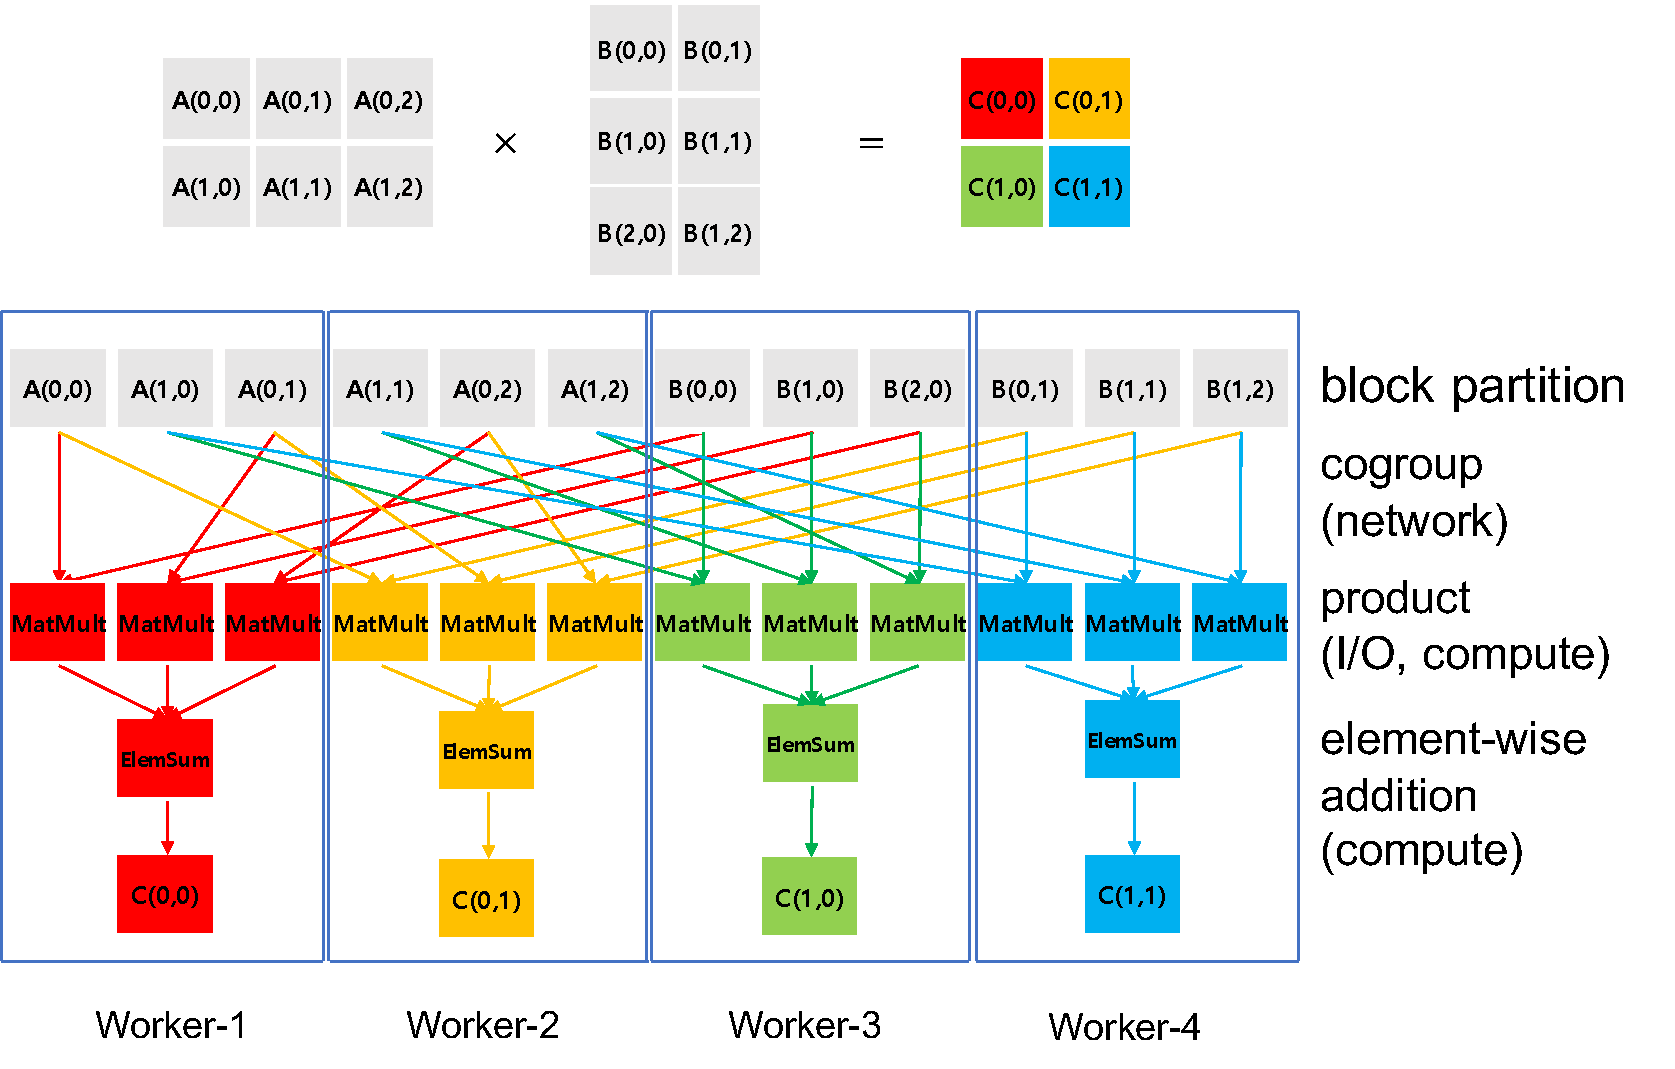
\includegraphics[width=0.5\textwidth]{figures/matmult-overhead-non-square-1.pdf}\caption{Block-based distributed matrix multiplication and its overhead in each step. Network, I/O, and CPU are principal resources for the execution.}\label{fig:matmul-with-overhead}
\end{figure}

\section{Matrix Multiplication on a Distributed Computing Environment}\label{sec:distributed-matrix-computation}
Optimization of distributed matrix multiplication is well studied in the literature. In the HPC community, many works focused on minimizing communication cost using the MPI model. Representative works include SUMMA~\cite{summa} and CARMA~\cite{carma}. Despite of the performance optimality of the methods, they have limitations regarding the programmability, scalability, and robustness comparing to general purpose big data analysis systems, such as Spark~\cite{spark} and Hadoop~\cite{hadoop}, especially on a shared cloud computing environment.

Apache Spark is an open source big data analysis platform. The primary abstraction in Spark is Resilient Distributed Dataset (RDD), which represents a read-only collection of objects partitioned across a set of machines. Spark manages large-scale data using partitions that help parallelize distributed data processing while guaranteeing the fault-tolerance with lineage and task execution optimization with lazy evaluation~\cite{spark}.

In Spark, matrix-related linear algebraic operations are supported in the MLlib library~\cite{spark-mm} with various matrix partitioning schemes (row-, column-, and block-based) and a set of distributed operation APIs on the matrix. To multiply two matrices, Spark MLlib automatically identifies the optimal way of task distribution based on the input matrix partitioning scheme and uses Scala Breeze library to execute multiplication. Let us give an example of multiplying two matrices, $C = A \times B$. If $A$ is row-partitioned and $B$ is column-partitioned, the Cartesian product is performed for each row block of $A$ and column block of $B$. If both $A$ and $B$ are block-partitioned, the block dimension of result matrix, $C$, is decided by considering the number of workers and input block dimensions. A work node that is responsible for each resulting block fetches all the necessary blocks from $A$ and $B$ to execute multiply operation locally.


Figure~\ref{fig:matmul-with-overhead} shows an example of block-based matrix multiplication. A left matrix, $A$, is block-partitioned by $2 \times 3$, a right matrix, $B$, is partitioned by $3 \times 2$, and the result matrix, $C$, is partitioned by $2 \times 2$. In Spark, a \textit{cogroup} operation by the result matrix block index allows a worker node that is responsible for a result block to collect necessary left and right matrix blocks. During \textit{cogroup} operation, network overhead is dominant. After collecting all necessary blocks, each worker node performs product operations followed by element-wise additions. In the step, I/O overhead to read the fetched blocks from a \textit{local.dir} location and compute overhead dominate.

\subsection{Distributed Matrix Multiplication Overhead Modeling}\label{sec:overhead-modeling}
Dense matrix multiplication is widely known as a CPU intensive task, but other resource overheads become non-negligible when it is executed on a large-scale distributed computing environment, such as Spark. To qualitatively understand characteristics of a distributed matrix multiplication task, we summarize IO, network, and compute overheads. Let us assume the number of rows of a left matrix as $LR$, the number of columns of a left matrix (or the number of rows of a right matrix) as $LC$, and the number of columns of a right matrix as $RC$. Accordingly, the result matrix size is $LR \times RC$. Left, right, and result matrices are block-partitioned whose block size is expressed in the lowercase letter ($lr$, $rc$, and $lc$, where $LR \geq lr$, $LC \geq lc$, and $RC \geq rc$).

\textbf{Shuffle}: A worker node that is responsible for computing an output matrix block of size $lr \times rc$ has to fetch blocks from left and right matrices with the size of $lr \times LC$ and $LC \times rc$, respectively. If a worker node does not contain required blocks locally, it has to fetch them from remote machines that incur network overhead. Assuming uniform block distributions among workers, the network overhead in the shuffle phase can be expressed as Equation~\ref{eq:shuffle-overhead}.
\begin{equation}\label{eq:shuffle-overhead}
  BlockFetchOverhead_{lr \times rc} \propto \sum\limits_{i=1}^{\frac{LC}{lc}} lr \times lc + lc \times rc
\end{equation}

\textbf{Compute}: After a shuffle step completes, a worker node performs multiplication of fetched blocks followed by element-wise addition. In order to perform multiplication, the blocks have to be read from a Spark local directory (\textit{spark.local.dir} configuration) that is generally set as a disk storage device. Thus, the I/O read overhead is same as the shuffle overhead and expressed as Equation~\ref{eq:shuffle-overhead}.

After loading the input matrix blocks into memory, each worker node executes a multiplication task whose overhead is expressed as Equation~\ref{eq:compute-overhead}.
\begin{equation}\label{eq:compute-overhead}
  ComputeOverhead_{lr \times rc} \propto \sum\limits_{i=1}^{\frac{LC}{lc}} lr \times lc \times rc
\end{equation}

In the element-wise addition step, the number of sum operation of each cell is proportional to $\frac{LC}{lc}$, and the size of each output block is $lr \times rc$.

\section{MPEC : Matrix Multiplication Performance Estimation}\label{sec:mpc-structure}
MPEC aims to predict the latency to complete multiplication of dense matrices that might have different size and shape. As the matrix multiplication is a core kernel task of many machine learning algorithms for big data analytics, we target to predict the performance on various cloud computing resources where many recent big data systems are deployed.

\begin{figure}
  \centering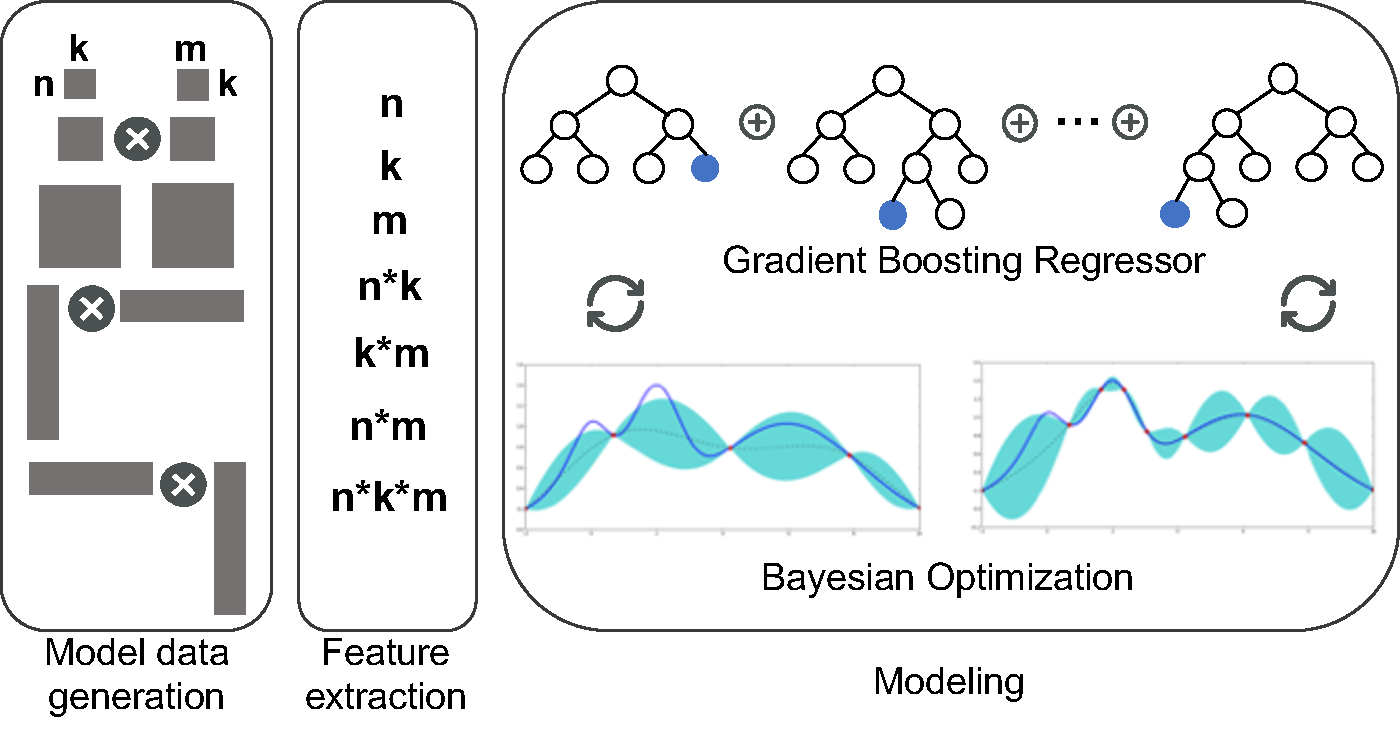
\includegraphics[width=0.5\textwidth]{figures/mpc-architecture.pdf}\caption{Architecture of MPEC to predict various matrix multiplication performance}\label{fig:mpc-architecture}
\end{figure}

The architecture of MPEC is shown in Figure~\ref{fig:mpc-architecture} that is composed of train dataset generation, feature extraction, and modeling. In the modeling step, we iteratively apply bayesian optimization~\cite{bayesian-optimization} to find the optimally working hyper parameters of the chosen modeling algorithm.

\subsection{Train Data Generation}\label{sec:train-data}
In the train data generation step, MPEC performs offline profiling of various types and sizes of matrix multiplication to build a model to predict latency of arbitrary input dataset. A matrix multiplication task can be broadly grouped into square $\times$ square, long-thin $\times$ short-wide, and short-wide $\times$ long-thin matrices. To cover all the shapes and various sizes, MPEC profiles the latency of synthetically generated left and right matrices. In the latency measurement, MPEC utilizes Apache Spark WebUI REST API that provides various execution metrics in the JSON format.

To get optimal performance from various cloud computing instances with distinct capacity, MPEC adopts OpenBLAS to conduct computation on CPU and NVBLAS to conduct computation on instances that equip GPU devices~\cite{NVBLAS}. To allow Spark to interact with the hardware-optimized linear algebra libraries, we use netlib-java as proposed in~\cite{fatman-littleboy}.

\subsection{Feature Extraction}\label{sec:features}
As shown in Section~\ref{sec:overhead-modeling}, overheads of matrix multiplication in a distributed computing environment encompass various sources of resources. In order to account for such diverse overheads, MPEC proposes to utilize the dimension of input matrix blocks and the products, namely $lr$, $lc$, $rc$, $lr \times rc$, $lr \times lc$, $lc \times rc$, and $lr \times lc \times rc$, as features to model the performance. With $lr \times rc$ term, we can consider the size of output matrix, $lr \times lc$ and $lc \times rc$ terms represent the size of left and right matrix blocks size that impacts network and I/O disk overhead. The $lr \times lc \times rc$ term represents the total number of multiply operations.

Different from MPEC, previous works that focus on predicting the performance of data mining tasks on cloud computing resources used a scale-based sampling mechanism as an input feature for prediction~\cite{ernest, cherrypick, paris}. They generally apply sampling at the input dataset by selecting very small portion and measure performance using the subset of the dataset. Using the outcomes from the sample dataset, they apply distinct predictive algorithms, such as non negative linear equation (Ernest~\cite{ernest}), bayesian optimization (Cherrypick~\cite{cherrypick}), and random forest (PARIS~\cite{paris}), to make a prediction. However, the scale-based sampling mechanism cannot capture the complex nature of distributed matrix multiplication, and it considers either $lr$ or $rc$ based on the sampling method. In the evaluation section, we demonstrate the superior performance of MPEC due to the rich set of features.

\subsection{Modeling}\label{sec:modeling}
In the modeling step, MPEC builds a model to represent the performance of multiplying various matrices. This step is composed of model build and hyper parameter search; MPEC utilizes Gradient Boosting~\cite{gradient-boosting} (GB) regressor for model build step and Bayesian Optimization~\cite{bayesian-optimization} to find the optimal parameters to run GB method.

Gradient Boosting~\cite{gradient-boosting} is a flexible non-parametric statistical learning approach for classification and regression. The main idea of GB is combining many weak learners that are generally applicable only to simple linear relations incrementally to model complex and non-linear interactions among features. A GB model is fitted in a forward stage-wise pattern; at each stage, a new weak learner model is fit to the residual of the current model, and it focuses more on correcting errors from the previous iterations. Different from a similar decision tree method, GB is known to be robust to overfitting by ensembling many weak learners~\cite{random-forest}.

When building a predictive model, properly setting model parameters is crucial to improve the quality of prediction. Many heuristics to search for the best performing hyper parameters are proposed, such as random walk, grid-based search, or using a statistical inference method. Among them, MPEC utilizes a statistical inference method based on the bayesian model~\cite{bayesian-optimization}. The bayesian optimization method searches for a set of next configuration values that are likely to improve model quality or to decrease uncertainty. It is a non-parametric black box approach that estimates an objective function (i.e., the complete performance measure from all combinations of parameters) using a stochastic process, such as Gaussian process. In predicting the objective function, bayesian optimization uses all of the information available from previous runs ($prior$), and the objective function model is updated ($posterior$) after new experiments are conducted ($likelihood$).

\section{Evaluation}{\label{sec:eval}}
In this section, we evaluate the performance of MPEC thoroughly with various cloud computing instance types, input matrix sizes, and shapes. In summary, applying gradient boosting algorithm with the proposed features outperforms linear regressor by showing 42\% more prediction accuracy. Furthermore, by applying bayesian optimization to select optimal hyper-parameters of gradient boosting, we could improve the accuracy about 2\%. Evaluation of MPEC with various cloud instance types demonstrates the effectiveness of MPEC on a cloud computing environment. Finally, comparing MPEC with Ernest~\cite{ernest}, the state-of-the-art machine learning performance predictor on cloud, shows that MPEC has about 16\% more accuracy in predicting matrix multiplication latency.

\subsection{Setup}
To make diverse matrix multiplication scenarios for evaluation, we generate left and right matrices with different number of rows and columns from 128 to 8,000,000. Within the range, we generate 236 synthetic test cases of square $\times$ square, long-thin $\times$ short-wide, and short-wide $\times$ long-thin matrices\footnote{test input cases - http://bit.ly/2CvOmnK}. The matrix multiplication is performed with Apache Spark and MLlib library with version 2.2.0. Multiplication of each matrix size is executed five times, and the median value is used to represent the latency for a task. A spark cluster is deployed to AWS EC2 by using \textit{spark-ec2} library\footnote{https://github.com/kmu-leeky/spark-ec2} with four \textit{R4.2xlarge} instances, unless otherwise stated. Each EC2 instance has hardware-optimized linear algebra library installed, namely NVBlas for a GPU instance (\textit{g2.2xlarge}) and OpenBlas for other instances. To apply modeling algorithms, we use \textit{scikit-learn} 0.18.1 with \textit{Python} 2.7.12. To evaluate the accuracy of prediction models, we use \textit{coefficient of determination} ($R^2$) as a metric. The metric is calculated as Equation~\ref{eq:cod}, and it measures how much the predicted outcome ($\hat{y_i}$) resembles the real measured value ($y_i$). The maximum value of the metric is $1.0$ that says the model predicts without an error (the larger, the better).

\begin{equation}\label{eq:cod}
  R^2 = \frac{\sum\limits_{i} (\hat{y_i}-\overline{y})^2}{\sum\limits_{i} (y_i-\overline{y})^2}
\end{equation}


\subsection{MPEC Performance Evaluation}
\subsubsection{feature importance} MPEC proposes to use various combinations of left and right matrix block sizes as features to model complex operation of distributed matrix multiplication. To assess the impact of proposed features in the gradient boosting regressor, we show the relative importance of features that are calculated by counting the number of times a feature is selected for splitting where each split is weighted by the improved performance~\cite{gb-feature-importance} in Figure~\ref{fig:feature-importance} gray bars. \emph{GradientBoostingRegressor} method is performed 100 times, and the average importance value is shown with the minimum and maximum value in the error bars. The total number of multiply operation ($lr \times lc \times rc$) term is the dominant feature (0.30) as people generally expect. However, a feature that represents the output matrix size ($lr \times rc$) and shuffle overhead ($lr \times lc + rr \times rc$) are also dominant factors, $0.25$ and $0.20$, respectively, and this observation corresponds to Figure~\ref{fig:different-matrix-shapes} that shows the latency might differ for matrix multiplication tasks with the same number of multiply operations but different shape and output size, e.g., long-thin $\times$ short-wide versus short-wide $\times$ long-thin. To quantitatively analyze the impact of each feature to the model accuracy, we show the coefficient of determination value in the secondary vertical axis. From the most important feature, we cumulatively add a next important feature (in the x-axis) and build a model. The best model accuracy is achieved with three most important features (the number of multiply operations, output matrix size, and the amount of shuffle overhead).

\begin{figure}
  \centering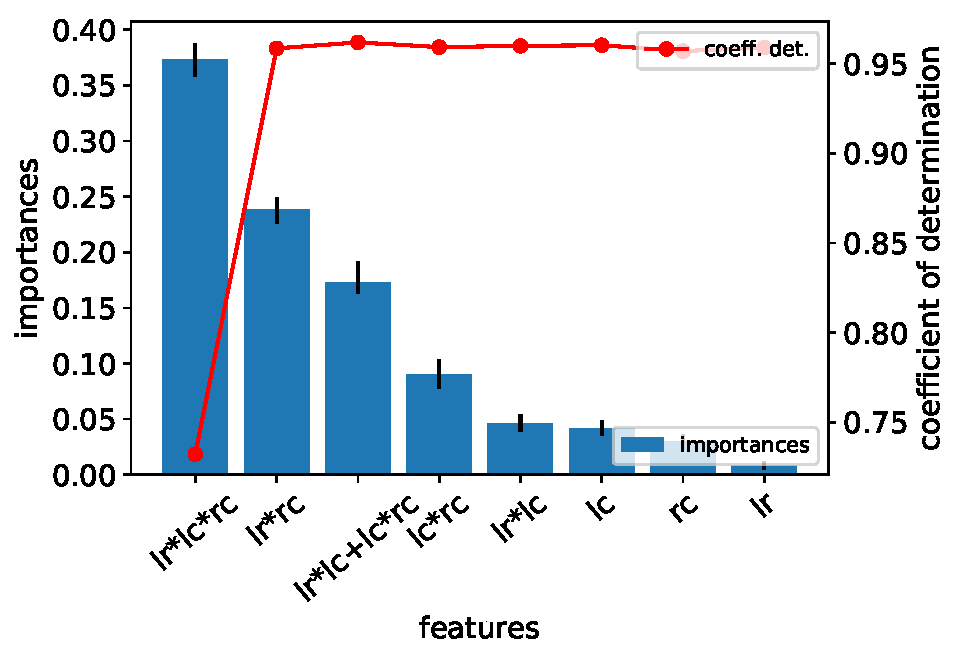
\includegraphics[width=0.45\textwidth]{figures/feature-importance.pdf}\caption{The relative importance of features and the impact to the model accuracy. The number of multiply operations, output matrix size, and  the shuffle overhead are the three most important features.}\label{fig:feature-importance}
\end{figure}

\subsubsection{effectiveness of bayesian optimization} MPEC uses bayesian optimization to find the optimal hyper parameters to build a model. To quantitatively analyze influence from the optimization step, we show three hyper parameters and the $R^2$ value in Table~\ref{table:bo-performance}. In the experiment, we use \textit{BayesianOptimization} library from \textit{bayes\_opt} package in Python. During optimization, we use 10-fold cross validation to generate train and test dataset and search for hyper parameters to maximize $R^2$ with 30 iterations. Comparing to default parameters of \textit{GradientBoostingRegressor}, the optimization step changes model parameters in the direction of increasing accuracy, i.e., more number of regression trees (n\_estimators), while controlling overfitting, i.e., avoid representing a case that is specific to a particular sample (min\_samples\_split). In the final row, we can see the accuracy of the model measured by the coefficient of determination increases slightly from $0.9586$ to $0.9689$.

\begin{table}
  \centering
  \begin{tabular}{|C{2.2cm}|C{1.5cm}|C{1.5cm}|}
  \hline
  &default&bayesian optimization\\
  \hline
  n\_estimators&100&114\\
  \hline
  min\_samples\_split&2&14\\
  \hline
  max\_features&8&6\\
  \hline
  performance ($R^2$)&0.9586&0.9689\\
  \hline
  \end{tabular}
  \caption{\label{table:bo-performance}Parameters suggested by optimization module and the improved performance}
\end{table}

\subsubsection{prediction algorithm comparison}
To achieve the goal of predicting latency of various sizes and shapes of matrix multiplication tasks, other machine learning algorithms can be applied with features that are proposed in this paper. Among the algorithms, we compare decision tree regression variant algorithms and a linear regression variant method. For the decision tree variant, we compare gradient boosting regressor that is introduced in Section~\ref{sec:modeling} and random forest~\cite{random-forest}. Different from gradient boosting, random forest regressor builds multiple regressor trees by randomly selecting features and samples. Both gradient boosting and random forest regressors represent the non-linear character of input data while preventing over-fitting by combining outcomes from many weak learners. As a linear regression variant method, we adopt non-negative least squares (NNLS) regressor. In predicting latency, the non-negativity constraint should be imposed to avoid the latency being less than zero, and NNLS finds the optimal linear model that minimizes the prediction error with the constraint.

Figure~\ref{fig:r2-comparison} shows the prediction accuracy of three different algorithms. For each algorithm, we utilize the input dataset and features that are presented in Section~\ref{sec:mpc-structure} and use 10-fold cross validation to split train and test dataset. 100 times of experiments are performed with different sets of train and test data, and the average value is plotted with the minimum and maximum value in the error bars. The gradient boosting regressor shows the best accuracy with the $R^2$ value of $0.968$, followed by random forest regressor and NNLS with the $R^2$ of $0.955$ and $0.869$, respectively. From the figure, we can see that the linear equation cannot capture the non-linear interactions among proposed features in this paper. Figure~\ref{fig:gbm-measured-predicted} (gradient boosting regressor) and Figure~\ref{fig:nnls-measured-predicted} (NNLS) show the measured latency and predicted latency in the x and y axis, respectively. The dotted line means the prediction with no error (slope of one), and scattered points close to the line are accurate predictions. From the figures, we can confirm that the gradient boosting regressor provides better accuracy in the latency prediction.

\begin{figure}[t]
  \centering
  \subfloat[latency prediction accuracy]{\label{fig:r2-comparison}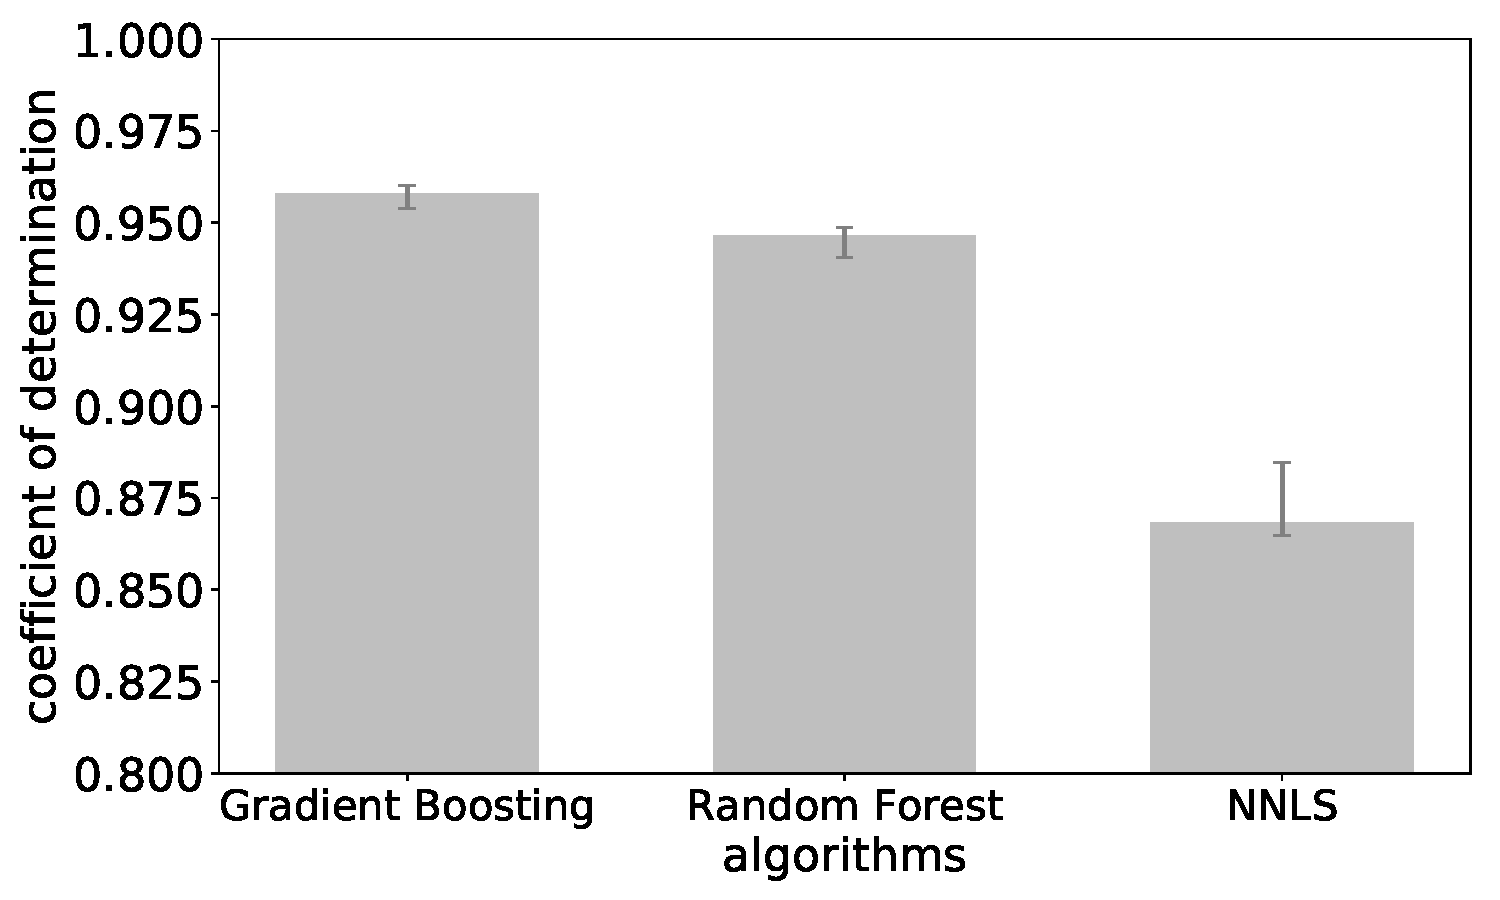
\includegraphics[width=0.4\textwidth]{figures/compare-algorithms.pdf}}\\
  \subfloat[gradient boosting regressor]{\label{fig:gbm-measured-predicted}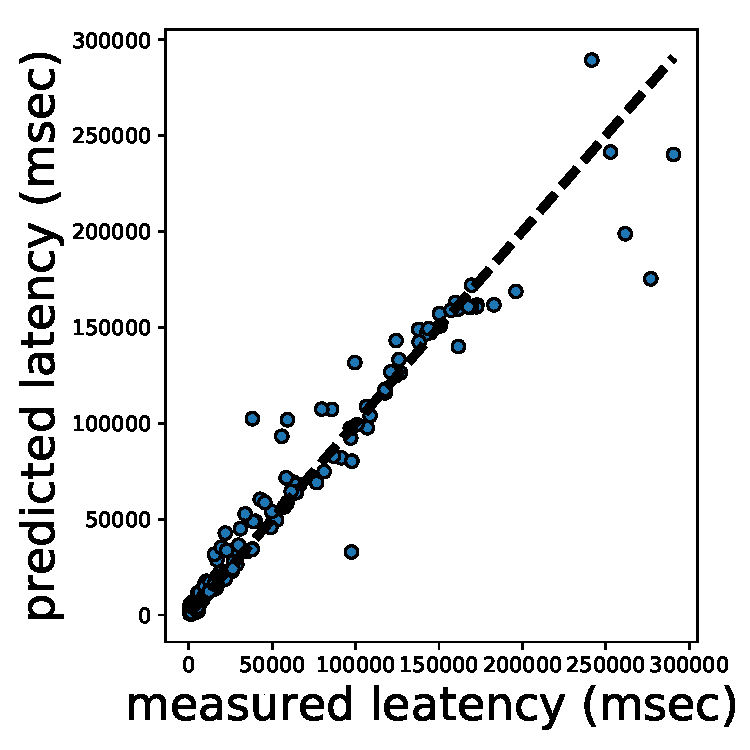
\includegraphics[width=0.23\textwidth]{figures/gbm-measured-predicted.pdf}} \hfil \subfloat[linear regressor]{\label{fig:nnls-measured-predicted}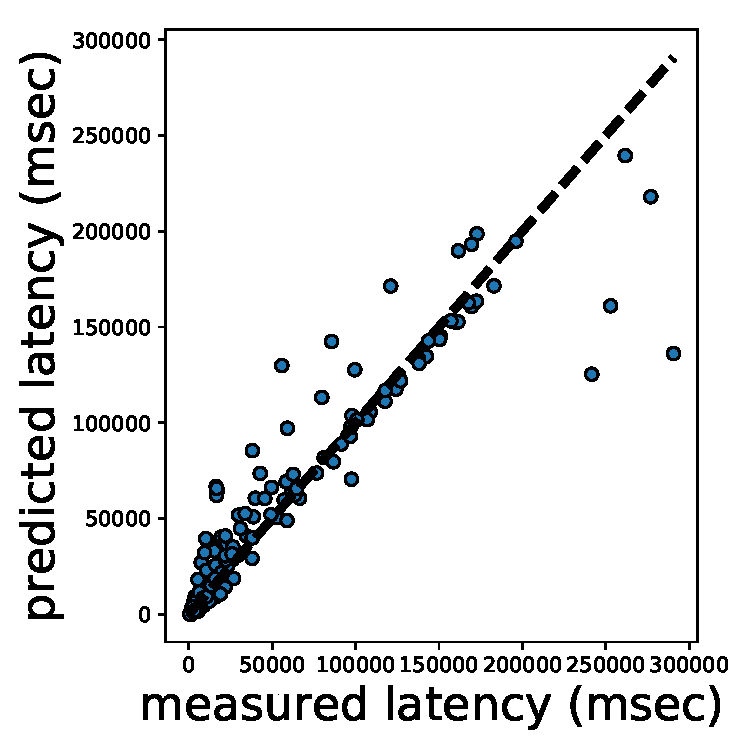
\includegraphics[width=0.23\textwidth]{figures/nnls-measured-predicted.pdf}}
  \caption{\label{fig:algorithm-comparison}Prediction accuracy comparison of various algorithms}
\end{figure}

\subsubsection{MPEC with various cloud computing instances}
In order to check the applicability of MPEC with various cloud computing instance types, we compare the performance of MPEC with compute-optimized EC2 instance (\textit{C4.2xlarge}), GPU instance (\textit{G2.2xlarge}), and memory-optimized instance (\textit{R4.2xlarge}). Despite of the same instance size (\textit{2xl}), different instances have distinct hardware configurations and hourly price. For example, the compute-optimized instance equips higher frequency processors with smaller RAM, and the memory-optimized instance provides larger RAM with lower CPU frequency. Due to the different memory size of instances, the maximum size of matrices for multiplication can differ. To make fair comparison, we select intersection of matrix sizes that can be processed in all three instance types. Input dataset generation and modeling step are conducted as presented in Section~\ref{sec:mpc-structure}. For the model accuracy evaluation, 10-fold cross validation is performed 100 times, and average $R^2$ value is presented in Figure~\ref{fig:gbm-diff-instances-r2-score} with error bars. We can see that regardless of instance types, the accuracy metric scores over $0.9$ and provides decent prediction accuracy.

To quantitatively understand the prediction accuracy of MPEC with different instance types, we show the latency of three representative workloads with different shapes in Figure~\ref{fig:gbm-measured-predicted-ticks}, namely short-wide $\times$ long-thin, square $\times$ square, and long-thin $\times$ short-wide. In each matrix multiplication workload, we show measured latency (gray bar) and predicted latency (gray bar with dots) per instance type. Despite of good prediction accuracy, the absolute latency value differs significantly across different instance types. For example, executing 128 $\times$ 5,000,000 $\times$ 128 matrix multiplication using \textit{G2} incurs over three times more latency than \textit{R4} instance. If we consider the price of two instances, as of writing \textit{R4.2xlarge} costs \$0.532 and \textit{G2.2xlarge} costs \$0.65 in the us-west-2 region, the gap becomes even larger. This experiment result demonstrates the importance of accurate latency prediction of matrix multiplication in order to appropriately choose cloud instances for big-data analysis workloads.

\begin{figure}[t]
	\centering
	\subfloat[latency prediction accuracy of different instance types]{\label{fig:gbm-diff-instances-r2-score}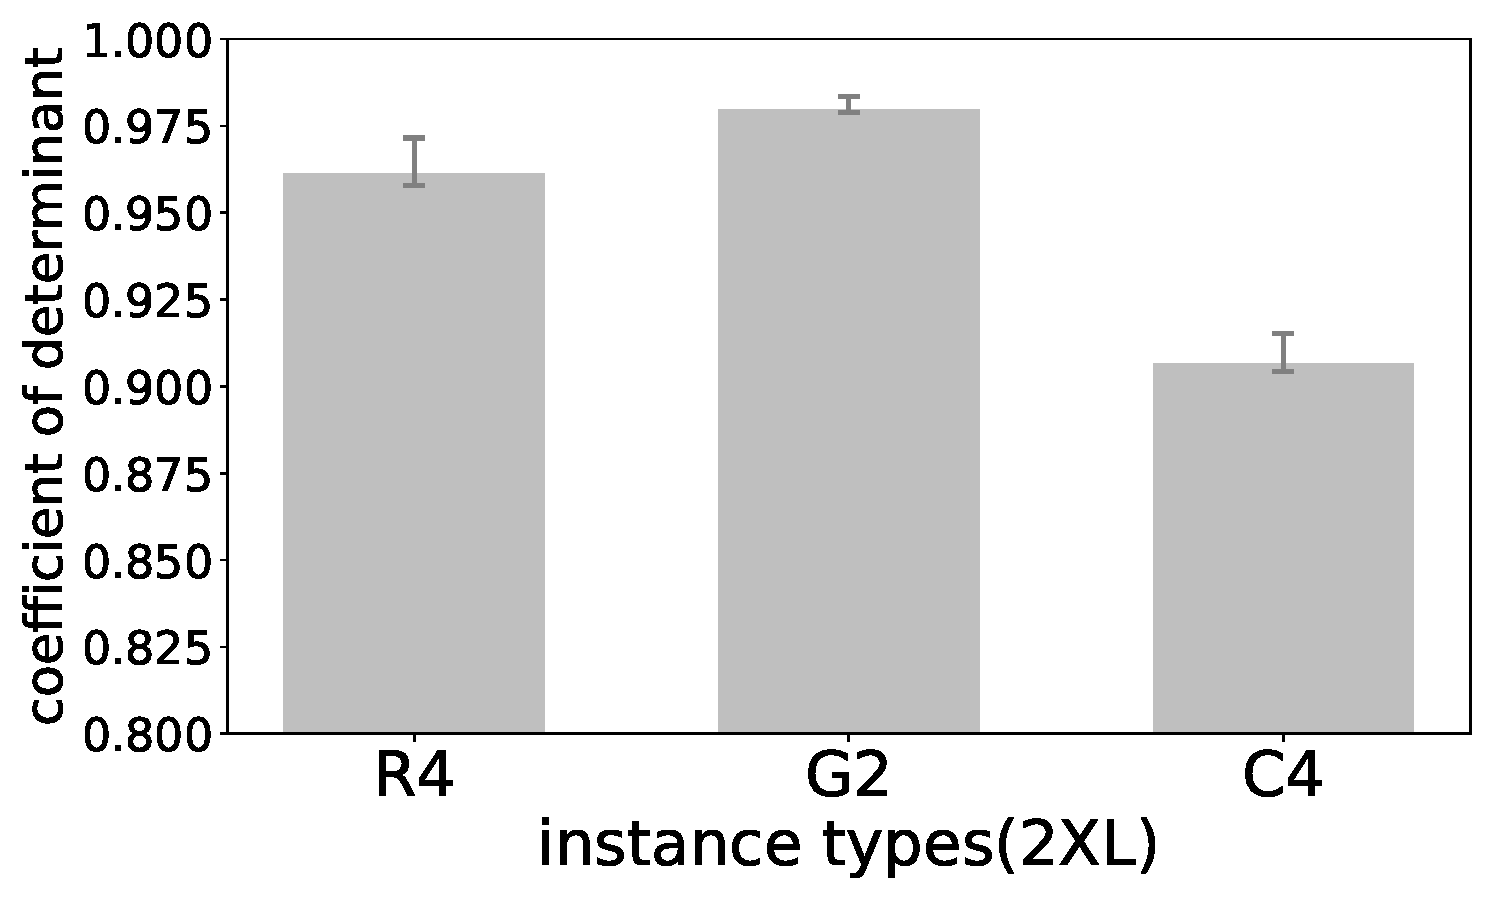
\includegraphics[width=0.4\textwidth]{figures/compare-instances-gbm-r2.pdf}}\\
	\subfloat[measured and predicted latency with different matrix shapes and instance types]{\label{fig:gbm-measured-predicted-ticks}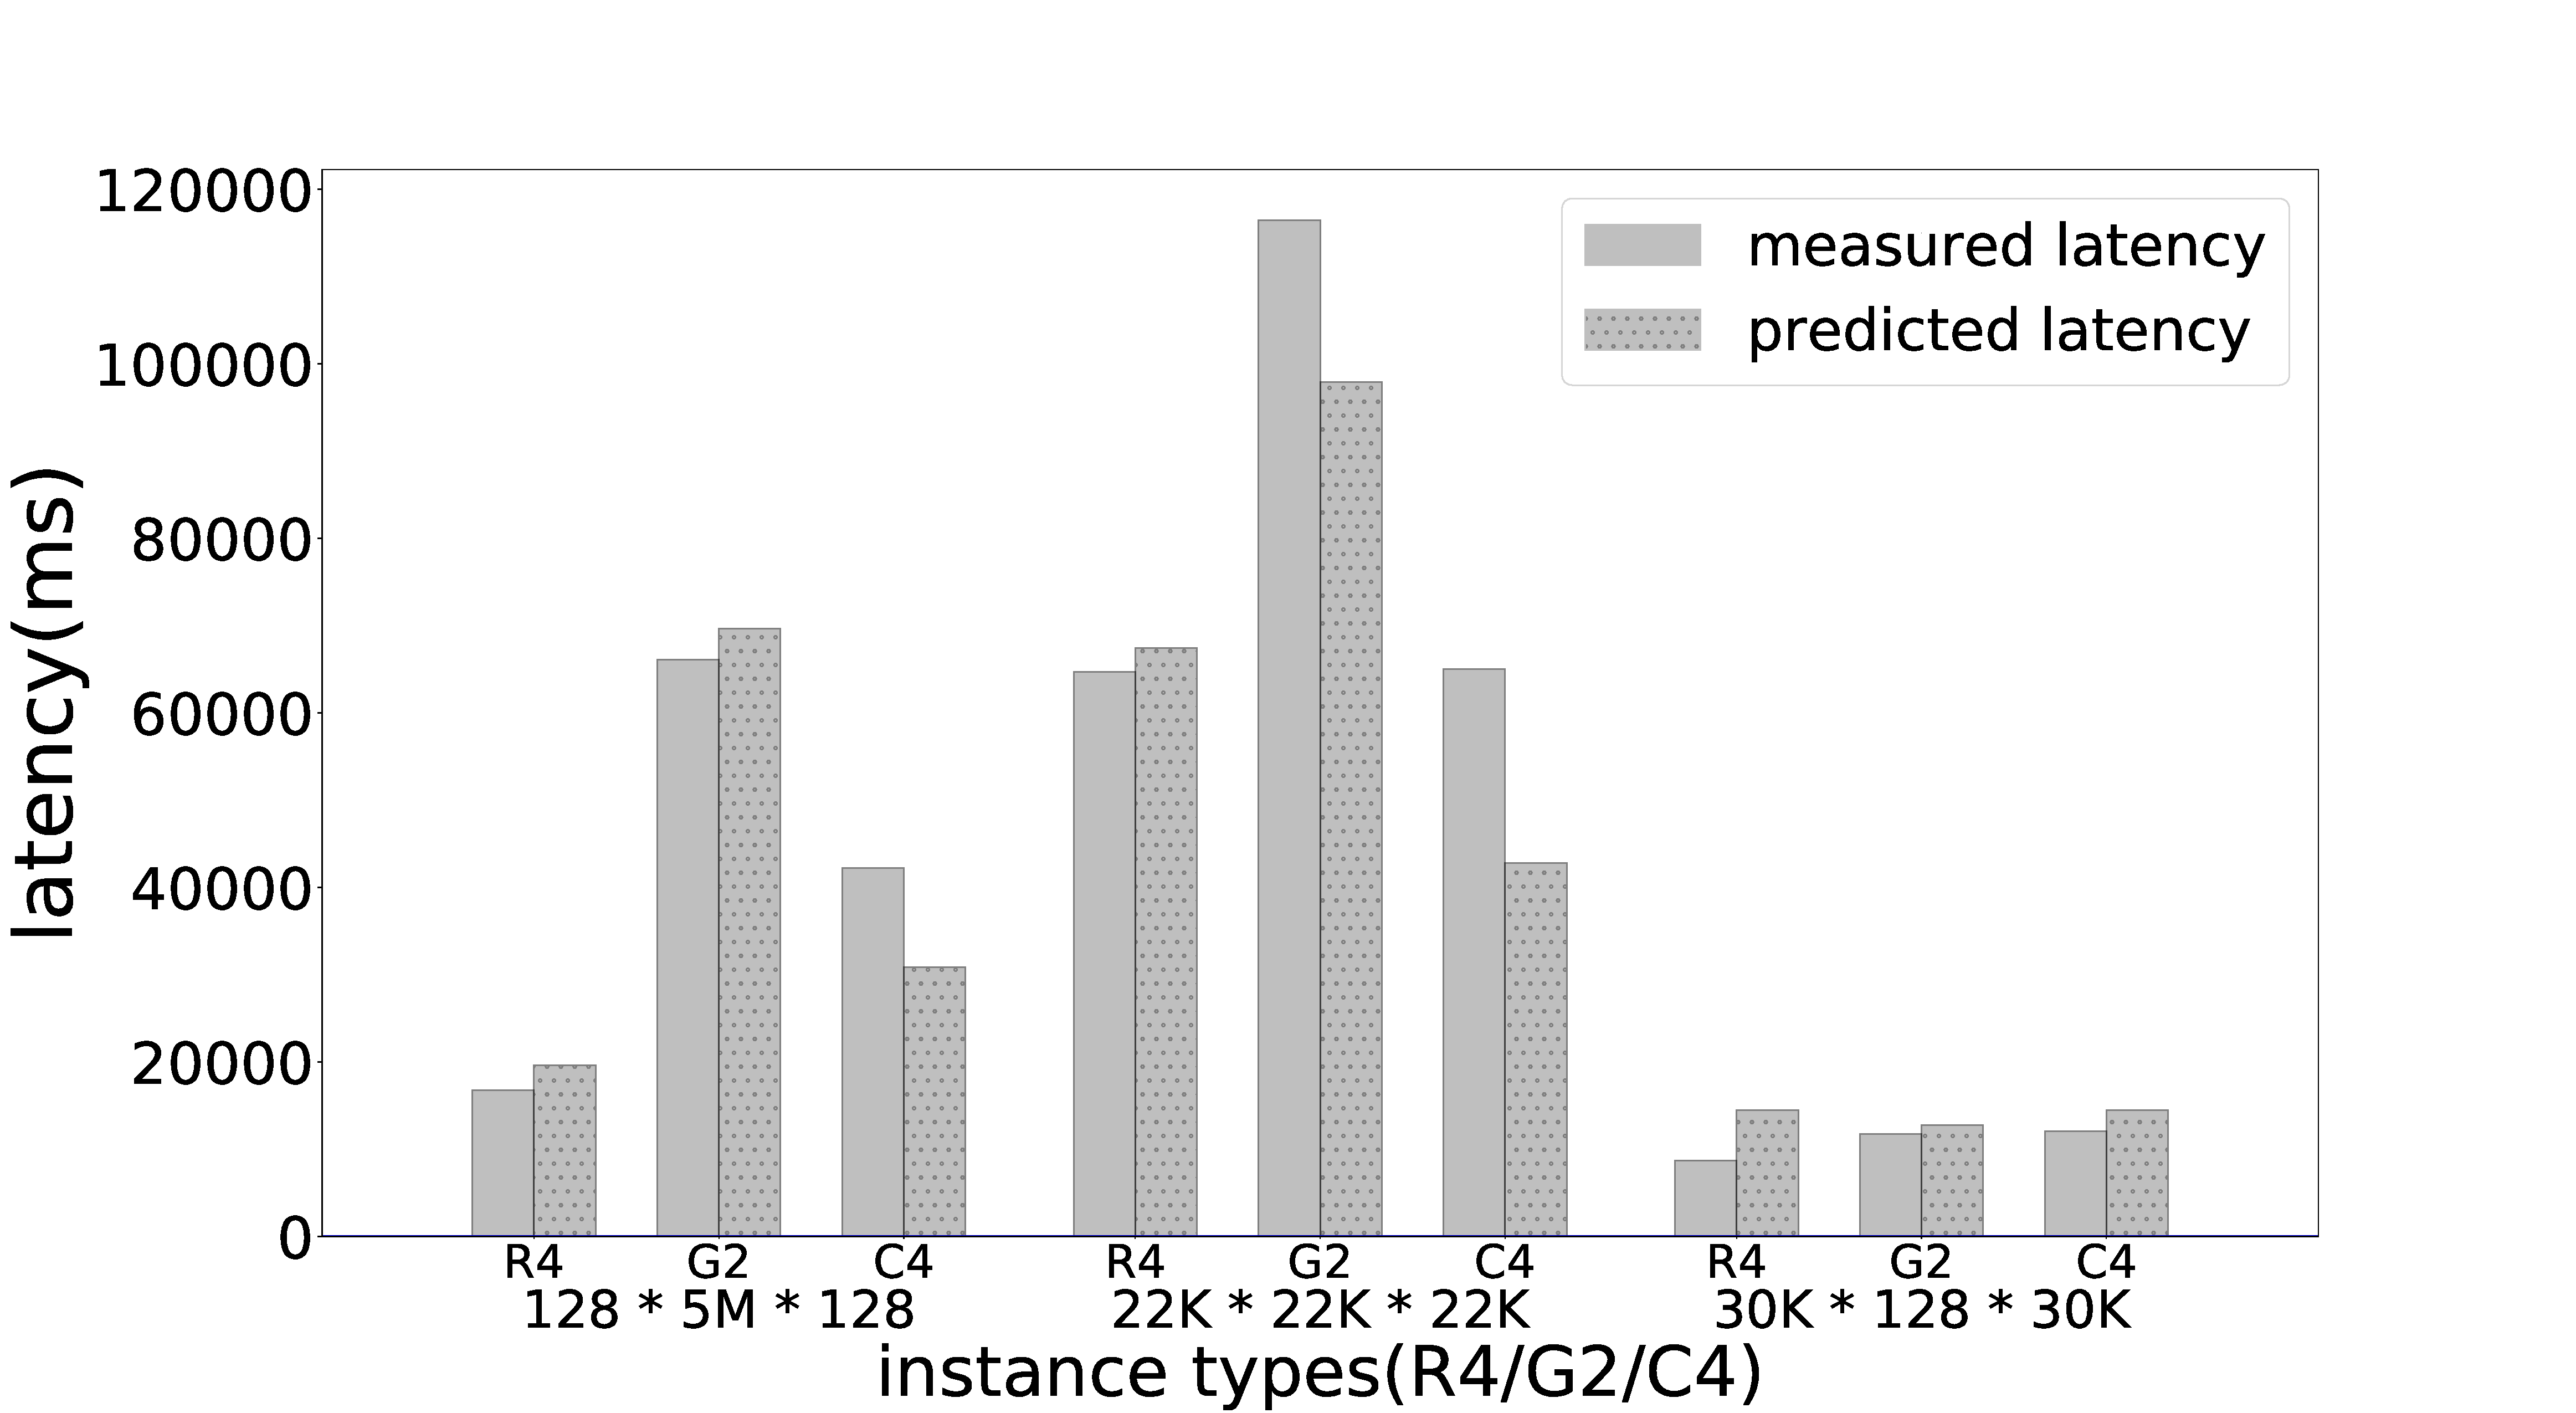
\includegraphics[width=0.5\textwidth]{figures/GBM-measured-predicted-ticks.pdf}} \hfil
	\caption{\label{fig:gbm-comparison}Performance of MPEC with different cloud computing instances}
\end{figure}

\subsubsection{Comparing MPEC with Ernest}
Ernest~\cite{ernest} is one of the most recent and accurate work that provides cloud computing instance recommendation for various machine learning tasks. Ernest is composed of two steps, experiment design and performance prediction. In the experiment design step, Ernest builds test cases with small fraction of sampled dataset and distinct number of machines to run experiments. In the prediction step, it uses a linear regressor with the non-negativity constraint and metrics gathered from experiments. In order to apply matrix multiplication tasks to Ernest, we should define the workload fraction to enable sampling, but there is no clear way to scale-down matrix multiplication workload. Due to the limitation, we apply Ernest in two ways. One is to divide the number of elements (number of rows $\times$ number of columns) in the left and right matrix by the fraction - \textit{Ernest-Element}. Another way is to scale-down the workload by the total number of multiply operations (number of left matrix rows $\times$ left matrix columns $\times$ right matrix columns) - \textit{Ernest-Multiply}. We choose three representative matrix shapes, namely square $\times$ square, long-thin $\times$ short-wide, short-wide $\times$ long-thin, with the largest matrix size available for execution with four \textit{R4.2xlarge} machines. While performing Ernest experiments, some test cases could not complete due to memory constraints, and it presents inaccuracy of Ernest when generating test cases.

The experiment result is shown in Figure~\ref{fig:mpc-ernest}. For different matrix shapes, we show the true measured value, the predicted latency of MPEC, Ernest-Element, and Ernest-Multiply from left to right bars. Ernest prediction model shows poor accuracy comparing to MPEC except a workload of 128 $\times$ 8,000,000 $\times$ 128, regardless of workload scale-down mechanisms. On average, the prediction accuracy of MPEC is better than Ernest-Element by 28\% and 37\% than Ernest-Multiply. Other than the poorer prediction accuracy of Ernest than MPEC, furthermore, Ernest cannot reuse experiment results from other matrix multiplication tasks as the experiment design of Ernest requires scaling down the original workloads precisely by the dataset fraction and number of machines. Different from Ernest, MPEC can reuse result of other matrix multiplication tasks to make the input dataset pool larger to improve model accuracy with diverse cases of matrix multiplication tasks.

\begin{figure}[t]
	\centering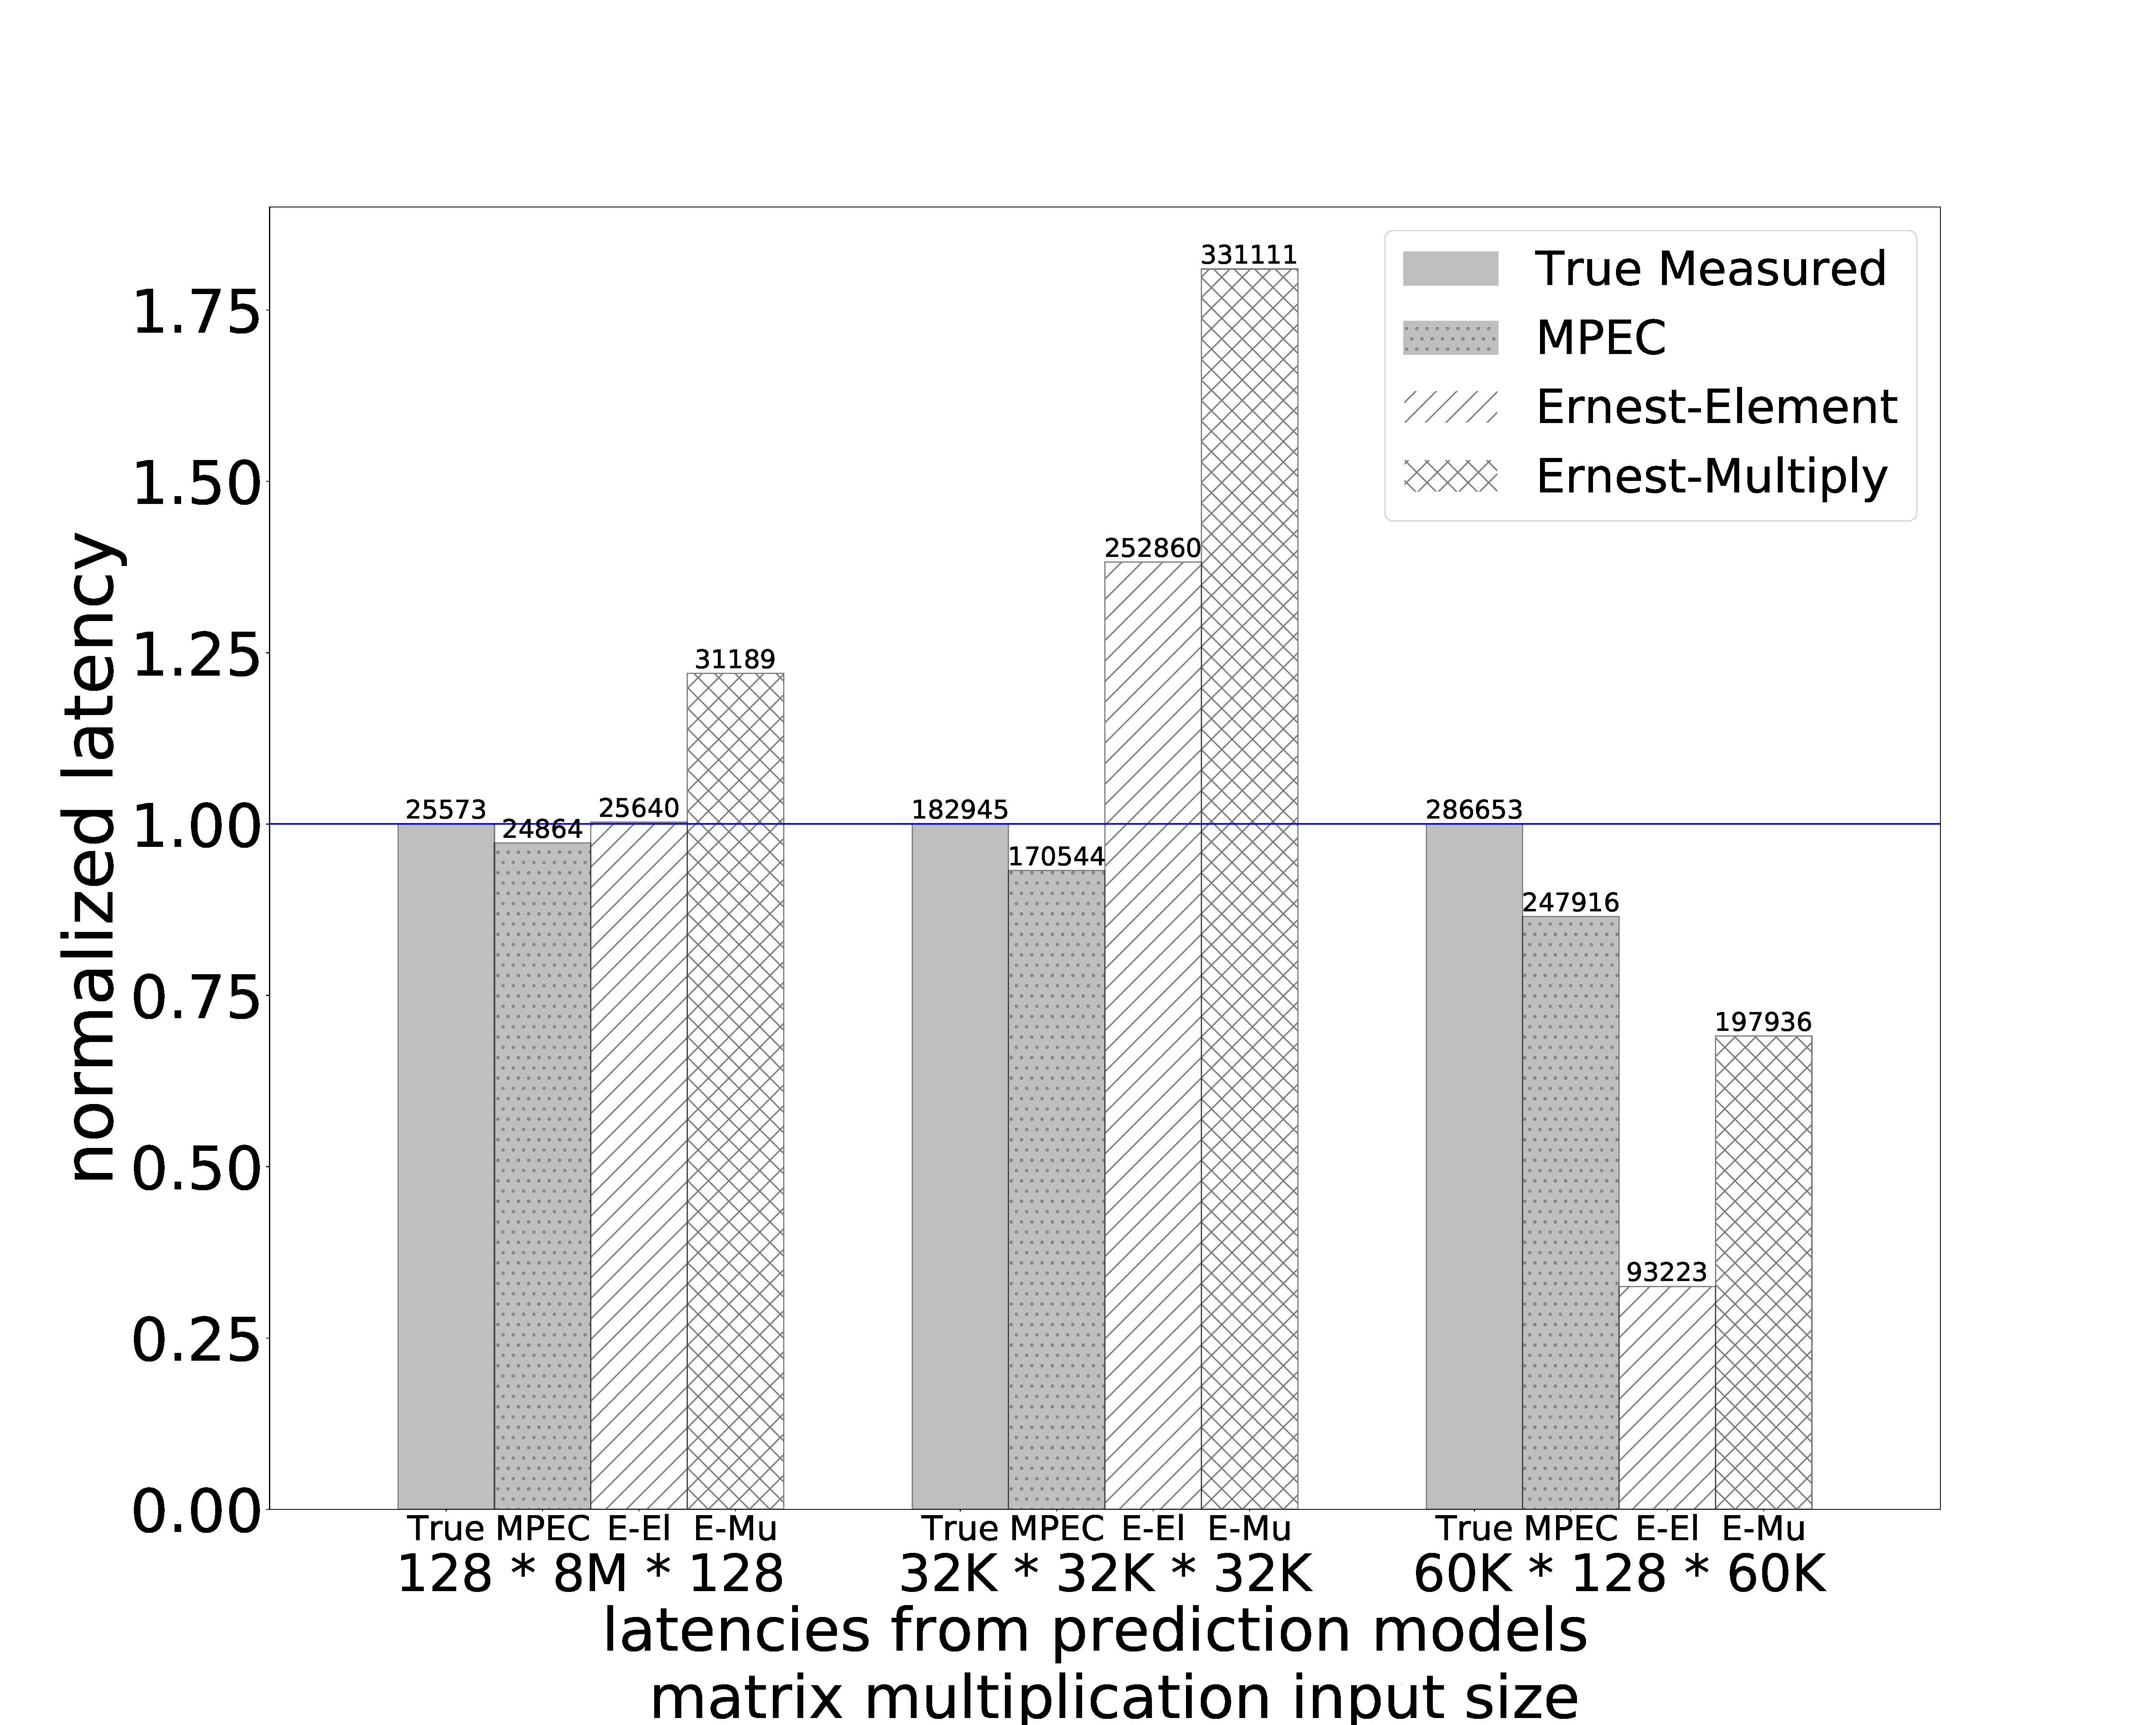
\includegraphics[width=0.5\textwidth]{figures/MPC-Ernest-compare.pdf}\caption{Comparing MPEC with Ernest}\label{fig:mpc-ernest}
\end{figure}

\section{Related Work}\label{sec:relatedwork}
\textbf{Big data workload performance estimation on cloud}: In a cloud computing environment, there are a large number of instance types that have unique hardware configurations, and few works propose a method to build an optimal environment to run big data analysis  workloads. Ernest~\cite{ernest} proposes a method to predict performance of arbitrary data mining algorithms with different number of workers on cloud. The proposed algorithm is composed of two parts, an experiment design step to select candidates of input data set to perform profiling and a prediction step to calculate the expected latency with a different number of resources. PARIS~\cite{paris} takes a hybrid online/offline approach, using a random forest model to predict application performance on various VM configurations based on features such as CPU utilization obtained from profiling. Cherrypick~\cite{cherrypick} proposes to use bayesian optimization to select instance type candidates to perform off-line profiling to predict performance on various cloud instance types. Those works rely on a scale-based sampling method for a given input dataset, and the profiled result is not reusable for other input datasets. Furthermore, they focus on predicting high-level machine learning algorithm execution latency and cannot capture the complex nature of a distributed matrix multiplication task. Thus, the prediction accuracy drops as they are applied to an algorithm whose kernel is distributed matrix multiplication.

FiM~\cite{fim} estimates the running time of iterative and multi-stage HPC applications on cloud by modeling the status of CPU cycles using a Stochastic Markov model. To estimate the parameters of the model, it uses linear regression. Similar to FiM, Mariani et. al.~\cite{hpc-cloud-predict} proposes a machine-learning based modeling method to predict HPC application performance on cloud. It first profiles the behavior of an application by using hardware-independent metrics, and it runs the application on a few cloud instances and measures the performance. The correlation between application metrics and the cloud instance is discovered by using the Random Forest algorithm. The previous two works rely on sampling of applications or input dataset, and a model is not reusable for new dataset. In MPEC, we measure the latency of performing matrix multiplication of arbitrary sizes, and the previous experiment result can be used to improve prediction accuracy of any input.

\textbf{Optimizing distributed matrix multiplication on cloud}: The matrix multiplication is an important task when running machine learning jobs with a large-scale dataset. Due to the importance of the task and the ever-increasing dataset to process, many works focused on optimizing the task on a distributed cloud computing environment. Yu et. al.~\cite{matmult-overhead-profiling} thoroughly investigates communication overhead of various shapes of distributed matrix multiplication and proposed few task execution plan to minimize communication cost. Marlin~\cite{marlin} proposes a distributed matrix multiplication algorithm on Spark to minimize shuffle overheads. As quantitatively discussed in this paper, the shuffle overhead is crucial to decide the performance of distributed matrix multiplication tasks. However, other than the shuffle overhead, the output matrix size and the total number of product operation also impose significant impact to the overall task completion time as presented in this work.

\section{Conclusion and Future Work}
In this paper, we presented MPEC, Matrix Multiplication Performance Estimator on Cloud Computing, that predicts execution time of distributed matrix multiplication with various input dataset on diverse cloud computing instances. We first characterize overheads of distributed matrix multiplication and propose eight features that represent different steps of the task. In the modeling step, we propose to use gradient boosting regressor to model non-linear interactions among features and bayesian optimization to find better performing hyper-parameters in an efficient way. We evaluated over 200 cases of various matrix multiplication scenarios (square $\times$ square, long-thin $\times$ short-wide, short-wide $\times$ long-thin) on various cloud computing instances. The evaluation reveals that among the proposed features, the number of product operations, the output matrix size, and shuffle overhead are three most important features to decide overall latency. Performance comparison to the state-of-the-art cloud computing performance predictor, Ernest, reveals that MPEC provides 16\% more accurate result when predicting latency of distributed matrix multiplication task.

In this work, we confirm that accurate prediction of distributed matrix multiplication is feasible with well-represented features. On top of findings in this paper, we are actively working on selecting a small number of representative distributed matrix multiplication workloads that still provide high prediction accuracy while lessening the performance profiling overheads in different cloud computing instances. Beside eight features used for modeling task latency on MPEC, we plan to add more features of unique cloud computing instance configurations, such as clock rate, network bandwidth, and memory size. We expect that additional features would help to predict task latency of different types of cloud computing instances.
\bibliographystyle{IEEEtranS}
\bibliography{abc2}
\end{document}
